% TODO: try not to look down so much while talking
\documentclass[table]{beamer}
\usepackage{presentation}
\title{Generalizing Lenses}
\subtitle{A New Foundation for Bidirectional Programming}
\author{Daniel Wagner} % for hyperref
\date{June 13, 2014}

\begin{document}

% TODO: practice, word for word, your first few sentences
\author{Daniel Wagner\\[3ex]\img{0.2\linewidth}{plclub-logo}} % for beamer
\maketitle

\begin{frame}
    \frametitle{History: a problem with databases}
    \begin{diagram}[outer sep=1em]
        \path<+->
            node[DB]              (db)     {\phantom{DB}}
            node[right=6em of db] (result) {result}
            (db.base) node[anchor=base] {DB}
            (db) edge[->] node[above=-1em] (query) {query} (result)

            % dummies so things don't jump around from slide to slide
            node[DB,below=10.1ex of db,draw=none] {\phantom{DB}}
            (result.west) node[anchor=west] {\phantom{new result}}
            ;
        \path<+->
            node[below=10ex of db, DB] (db') {\phantom{DB}}

            (db' -| result.west)
            node[anchor=west] (result') {new result}

            (db'.base) node[anchor=base] {new DB}
            ;
        \path<.-.(1)>
            (db') edge[->] node[above=-1em] (query') {query} (result')
            (db)  edge[->] (db')
            ;
        \path<+>
            (db)  edge[draw=none]
                coordinate[right=1em,pos=0.9] (update base)
                node[right=1em, pos=0.3, thought,
                     callout absolute pointer=(update base)
                    ] (update) {\tiny result $\to$ new result}
            (db')
            ;
        \path<+>
            (result)  edge[draw=none] coordinate[pos=1] (above result') (result')
            (result)  edge[->] (result |- above result')
            (result') edge[->] node[above=-1em] (inverse) {reverse query} (db')
            ;
    \end{diagram}
\end{frame}

% TODO: Nicole says these next few slides did not go smoothly
\begin{frame}
    \frametitle{Bidirectional programming}
    Many other settings with similar problems, like
    \begin{itemize}
        \item parsing (in-memory structures $\leftrightarrow$ serialization),
        \item software model transformations (diagrams $\leftrightarrow$ code),
        \item user interfaces (connecting two widgets' state), and
        \item sysadmin (custom configurations $\leftrightarrow$ unified format).
    \end{itemize}

    In each setting,
    \begin{itemize}
        \item two pieces of data (henceforth, \emph{repositories}) are related, and
        \item we would like to avoid writing two related transformations.
    \end{itemize}
\end{frame}

% TODO: this slide needs some thought about what to say while it's up
% TODO: Nicole says I slowed down a bit when presenting this in the second
% practice run
\begin{frame}
    \frametitle{Dissatisfaction}
    Language-based research is centered on asymmetric lenses. But:

    \begin{description}[Misalignment]
        \item[Asymmetry] A canonical repository stores all information,
        \item[Misalignment] Lenses have limited access to information
            connecting old and new repositories, and
        \item[Performance] Traversing entire repositories requires high
            computation and memory resources.
    \end{description}

    \ldots though the extensive {\usebeamercolor{palette
    primary}\color{fg}syntax} is a key feature to keep.
\end{frame}

\begin{frame}
    \frametitle{Contributions}
    Symmetric lenses are the first lens framework that:
    \begin{itemize}
        \item Gives both repositories equal status
        \item Provide a computable sequential composition
        \item Retain modular reasoning principles
    \end{itemize}
    Edit lenses extend symmetric lenses with:
    \begin{itemize}
        \item Explicit representation of and computation with changes
        \item Support for incremental operation
        \item Behavioral laws constraining update
    \end{itemize}

    \vpause

    A prototype implementation explores the problem of generating change
    information.
\end{frame}

% TODO: related work we haven't discussed includes TGGs, C-lenses
% TODO: Nicole says, "You paused a lot while you looked at the table"
\begin{frame}
    \frametitle{Related work}
    \tiny
    \begin{tabularx}{\linewidth}{m{4.4em}|X|X|X|X}
        & Alignment & Symmetry & Performance & Syntax
        \\\hline
        algebraic       &\Y[edits]
                        &\N[no]
                        &\N[possibly, but unexplored]
                        &\N[not a goal]
        \\\hline
        matching        &\Y[mapping from holes to holes]
                        &\N[no]
                        &\N[repository and alignment information both
                        processed]
                        &\Y[variants of most AS-lens combinators]
        \\\hline
        annotated       &\Y[insertion, deletion, modification markers]
                        &\N[no]
                        &\N[alignment information includes repository]
                        &\Y[includes $\diag \in X \lens X \times X$]
        \\\hline
        asymm. $\delta$ &\Y[explicit alignments]
                        &\N[not a goal]
                        &\N[edits include repositories]
                        &\Y[via alternate framework]
        \\\hline
        symm. $\delta$  &\Y[edits]
                        &\Y[yes, but equiv. not explored]
                        &\N[edits include repositories]
                        &\N[alternate frameworks not instantiated]
        \\\hline
        const. maint.   &\Y[uninterpreted edits]
                        &\Y[yes; does not require equiv.]
                        &\N[no; all edits relative to $\init$]
                        &\Y[many primitives, but no composition]
        \\\hline
        \multicolumn{2}{c}{}% drop the vertical bar
        \\[-1.5ex]\hline
        symm. state     &\N[very bad]
                        &\Y[yes; requires equivalence]
                        &\N[no]
                        &\Y[mostly domain agnostic]
        \\\hline
        edit lenses     &\Y[edits]
                        &\Y[yes; requires equivalence]
                        &\Y[small edits support incremental operation]
                        &\Y[most standard lenses, and container map]
    \end{tabularx}

    \vpause

    \small
    \colorbox{accessiblegreen}{\strut green} means satisfies the objective,
    \colorbox{accessiblered}{\strut red} indicates some shortcomings
\end{frame}

\begin{frame}
    \frametitle{Other models of edits}

    \begin{itemize}
        \item $X \times X$ (before and after)
            \begin{itemize}
                \item State-based lenses
                \item[\ybullet] Very simple starting point
                \item[\nbullet] Not enough information about alignment
            \end{itemize}
        \item $X \to X$ (extensional edit operation)
            \begin{itemize}
                \item Stevens' algebraic study of delta lenses
                \item[\ybullet] Models many behaviors
                \item[\nbullet] Difficult to recover intensional data
            \end{itemize}
        \item category on $X$ (collection of edits for each before/after
            pair)
            \begin{itemize}
                \item Diskin, et al's delta lenses
                \item[\ybullet] Very rich information about change
                \item[\nbullet] Very rich information about change
            \end{itemize}
    \end{itemize}
\end{frame}

\begin{frame}
    \frametitle{Modules}
    Keep the best features of each: collection of edits for easy
    introspection + mapping to functions to cover many behaviors.

    \vpause

    Module $\left<X,\DX,\odot_X,\init_X\right>$ is:
    \begin{itemize}
        \item Set of values to be edited $X$
        \item Monoid of edits $\DX$
        \item Homomorphism from edits to operations $\odot_X \in \DX \to X
            \partialto X$
        \item Default value $\init_X$ is a technical detail; explanation
            later
    \end{itemize}

    \begin{pronunciation}
        \D & changes to \\
        \odot & apply \\
        \init & initial value \\
        \partialto & partial function to
    \end{pronunciation}
\end{frame}

\begin{frame}
    \frametitle{Monoids}
    Quick review: monoid means
    \begin{itemize}
        \item There is an identity $\ONE$
        \item and an associative binary operation (juxtaposition).
    \end{itemize}

    Homomorphisms $f$ respect this structure.
    \[f(\ONE) = \ONE\]
    \[f(m\;n) = f(m)\;f(n)\]
    In particular, for edits: identity always succeeds and does nothing, and
    edits can be run in sequence.

    \begin{pronunciation}
        \ONE & identity \\
        m\;n & $m$ times $n$
    \end{pronunciation}
\end{frame}

\begin{frame}
    \frametitle{Partiality}
    \[\odot_X \in \DX \to \alert<2>{X \partialto X}\]

    \pause

    \alt<2>{Why not just do nothing instead of failing?}%
           {Requiring totality forces you to include unnatural edits.}

    \pause

    \[M \triangleq \{\ONE\} \cup \{a \mapsto b \mid a,b \in \nat\}\]

    With totality:
    \begin{align*}
        (a \mapsto b)\;(b \mapsto c) \odot a &= c \\
        (a \mapsto b)\;(b \mapsto c) \odot b &= c
    \end{align*}
    \ldots must expand $M$ to accommodate this.

    With partiality, can define
    \[(a \mapsto b)\;(b \mapsto c) \triangleq a \mapsto c\]

    \begin{pronunciation}
        \triangleq & is defined equal to \\
        \mapsto & becomes
    \end{pronunciation}

    \pause
    Theorem: Partiality is an illusion.
\end{frame}

\begin{frame}
    \frametitle{Data structures}

    Common approach to implementing complex data structures:

    \[\tau := 0 \mid 1 \mid X \mid \tau+\tau \mid \tau\times\tau
           \mid \fix X\tau {\color<2->{lightgray}\mid \tau\to\tau}\]

    Try to design edit modules for each of these types.

    \vpause

    \uncover<3>{\alert{Does not work well.}}
\end{frame}

\begin{frame}
    \frametitle{Products}
    How to edit $X \times Y$? Either edit $X$ or edit $Y$.

    \begin{diagram}
        \node[matrix of nodes
             ,ampersand replacement=\&
             ] (pairs) {
                Cats $\times$ Dogs                \&
                \vimg{2em}{without_scarf}         \&[4em]
                \vimg{2em}{with_scarf}            \\
                \vimg{2em}{without_hat}           \&
                \pair{without_hat}{without_scarf} \&
                \pair{without_hat}{with_scarf}    \\[6ex]
                \vimg{2em}{with_hat}              \&
                \pair{with_hat}{without_scarf}    \&
                \pair{with_hat}{with_scarf}       \\
            }

            ($(pairs-3-2.south)!0.5!(pairs-3-3.south)$) node[below]
                {%
                    \strut%
                    \only<2>{$\mlleft{\mbox{+hat}}$}%
                    \only<3>{$\mlright{\mbox{+scarf}}$}%
                }
            ;
        \path<2>
            (pairs-2-2)     edge[->]                  (pairs-3-2)
            (pairs-2-3)     edge[->]                  (pairs-3-3)
            (pairs-3-2.225) edge[->] node {\nbullet} +(-0.5,-0.5)
            (pairs-3-3.315) edge[->] node {\nbullet} +( 0.5,-0.5)
            ;
        \path<3>
            (pairs-2-2)     edge[->]                  (pairs-2-3)
            (pairs-3-2)     edge[->]                  (pairs-3-3)
            (pairs-2-3.315) edge[->] node {\nbullet} +( 0.5,-0.5)
            (pairs-3-3.315) edge[->] node {\nbullet} +( 0.5,-0.5)
            ;
    \end{diagram}
\end{frame}

\begin{frame}
    \frametitle{Sums}
    % TODO: for dogs, perhaps age them instead of adding an accessory
    \begin{diagram}
        \node[matrix of nodes
             ,ampersand replacement=\&
             ,column sep=8em
             ,nodes={anchor=center}
             ] (pictures) {
                \strut Cats \&
                \strut Dogs \\
                \img{4em}{without_hat}   \&
                \img{4em}{without_scarf} \\[4ex]
                \img{4em}{with_hat}      \&
                \img{4em}{with_scarf}    \\
            }

            ($(pictures-1-1)!.5!(pictures-1-2)$) node (plus) {\strut +}
            (plus |- pictures-3-1.south) node[below]
                {
                    \strut%
                    \only<2>{$\mlstayl{\mbox{+hat}}$}%
                    \only<3>{$\mlstayr{\mbox{+scarf}}$}%
                    \only<4>{$\mlswitchlr\ONE$}%
                    \only<5>{$\mlswitchlr{\mbox{+scarf}}$}%
                    \only<6>{$\mlswitchll\ONE$}%
                }

            (pictures-2-1.west) +(-1.5,0) node (spacer-l) {}
            (pictures-2-2.east) +( 1.5,0) node (spacer-r) {}
            ;

        \path<2>
            (pictures-2-1)     edge[->]                  (pictures-3-1)
            (pictures-3-1.225) edge[->] node {\nbullet} +(-0.5,-0.5)
            (pictures-2-2.315) edge[->] node {\nbullet} +( 0.5,-0.5)
            (pictures-3-2.315) edge[->] node {\nbullet} +( 0.5,-0.5)
            ;
        \path<3>
            (pictures-2-1.225) edge[->] node {\nbullet} +(-0.5,-0.5)
            (pictures-3-1.225) edge[->] node {\nbullet} +(-0.5,-0.5)
            (pictures-2-2)     edge[->]                  (pictures-3-2)
            (pictures-3-2.315) edge[->] node {\nbullet} +( 0.5,-0.5)
            ;
        \path<4>
            (pictures-2-1)     edge[->]                  (pictures-2-2)
            (pictures-3-1)     edge[->]                  (pictures-2-2)
            (pictures-2-2.315) edge[->] node {\nbullet} +( 0.5,-0.5)
            (pictures-3-2.315) edge[->] node {\nbullet} +( 0.5,-0.5)
            ;
        \path<5>
            (pictures-2-1)     edge[->]                  (pictures-3-2)
            (pictures-3-1)     edge[->]                  (pictures-3-2)
            (pictures-2-2.315) edge[->] node {\nbullet} +( 0.5,-0.5)
            (pictures-3-2.315) edge[->] node {\nbullet} +( 0.5,-0.5)
            ;
        \path<6>
            (pictures-2-1)     edge[loop right]          (pictures-2-1)
            (pictures-3-1)     edge[->]                  (pictures-2-1)
            (pictures-2-2.315) edge[->] node {\nbullet} +( 0.5,-0.5)
            (pictures-3-2.315) edge[->] node {\nbullet} +( 0.5,-0.5)
            ;
    \end{diagram}
\end{frame}

\begin{frame}
    \frametitle{Sums, recap}
    Six kinds of sum edit for $X + Y$:
    \begin{center}
        $\mlstayl\dx$

        $\mlswitchll\dx$

        $\mlswitchrl\dx$

        \vspace{2ex}

        $\mlstayr\dy$

        $\mlswitchlr\dy$

        $\mlswitchrr\dy$
    \end{center}
\end{frame}

% TODO: I think can steal some slides explaining why alignment is
% important/hard to put here. Otherwise maybe it's hard to justify why
% ``rewrite the list elements'' isn't a good replacement for ``reorder the
% list'' later.

\begin{frame}
    \frametitle{Inductive types}
    First idea: $\D(\fix X\tau)\simeq\D(\tau[\fix X\tau/X])$.

    For lists with elements from module $A$, i.e. $\fix X1+A \times X$:

    \begin{description}[$\mlstayr{\mlright\dx}$]
        \item[$\mlstayl\anything$] Do nothing to the currently empty list.
        \item[$\mlswitch_{\anything L}(\anything)$] Delete the entire list.
        \item[$\mlstayr{\mlleft{\d a}}$] Modify the head of the list.
        \item[$\mlstayr{\mlright\dx}$] Modify the tail of the list.
        \item[$\mlswitch_{\anything R}(\anything)$] Replace the current
            list.
    \end{description}

    \alert{No way to insert or delete in the middle of the list.}

    Information never migrates; can't swap list elements.

    \begin{pronunciation}
        \tau[X/Y] & replace $Y$ by $X$ in $\tau$
    \end{pronunciation}

    \pause

    More baroque approaches have other problems.
\end{frame}

\begin{frame}
    \frametitle{Containers}
    A standard container $\left<I,P\right>$ is
    \begin{itemize}
        \item A set of shapes $I$ and
        \item For each shape $i$, a set $P_i$ of positions.
    \end{itemize}
    An \emph{$X$-instance} $\left<i,f\right>$ of container $\left<I,P\right>$ is
    \begin{itemize}
        \item A shape $i \in I$ and
        \item A function $f \in P_i \to X$.
    \end{itemize}
\end{frame}

\begin{frame}
    \frametitle{Lists as containers}
    \begin{align*}
        I   &\triangleq \nat \\
        P_i &\triangleq \{0,\ldots,i-1\}
    \end{align*}

    \vpause

    The list $[3,6,2]$ is represented as the pair
    \[\left<\begin{array}{l@{\;}l@{\ }r@{}l}3,\lambda p.
        &\mbox{if}  &p=0\mbox{ then }&3\\
        &\mbox{elif}&p=1\mbox{ then }&6\\
        &\mbox{elif}&p=2\mbox{ then }&2
    \end{array}\right>\]

    \begin{pronunciation}
        \nat & natural numbers
    \end{pronunciation}
\end{frame}

\begin{frame}
    \frametitle{Container restrictions}
    Three important changes:

    \begin{itemize}
        \item Module of shape edits
        \item Universe of positions $P_U$
        \item Partial order $\le$ on shapes (with $P$ monotone)
    \end{itemize}
\end{frame}

% TODO: perhaps swap this slide with the previous one, and explode the edits
% into a few slides or an animation or something
% TODO: think about what to say on this slide
\begin{frame}
    \frametitle{Container module}
    \begin{align*}
        \D\left<I,P\right>_X
            \triangleq{}&
                \{\ml{mod}(p,\dx) \mid p \in P_U, \dx \in \DX\}
            \\ \mathrel{\cup}{}&
                \{\ml{ins}(\d i) \mid \d i\;i \ge i\mbox{ whenever defined}\}
            \\ \mathrel{\cup}{}&
                \{\ml{del}(\d i) \mid \d i\;i \le i\mbox{ whenever defined}\}
            \\ \mathrel{\cup}{}&
                \{\ml{swap}(\d i,f) \mid f_i \in P_{\d i\;i} \simeq P_i
                \mbox{ whenever defined} \}
            \\ \mathrel{\cup}{}&
                \{\ml{fail}\}
    \end{align*}

    \begin{pronunciation}
        \simeq & bijection to
    \end{pronunciation}
\end{frame}

\begin{frame}
    \frametitle{Other results: composition}
    First in-depth study of machinery needed for sequential composition in
    the presence of symmetry:
    \begin{itemize}
        \item Complements enable computable composition
        \item Equality is too fine a distinction, but a coarser equivalence
            relation identifies $j;(k;\ell)$ and $(j;k);\ell$
        \item All lens combinators are proven to respect equivalence classes
        \item An induced category whose arrows are lenses
    \end{itemize}
\end{frame}

\begin{frame}
    \frametitle{Other results: algebraic study}
    For symmetric lenses:
    \begin{itemize}
        \item Symmetric monoidal product structure
        \item Symmetric monoidal sum structure
        \item \emph{Non}-existence of true products and sums
        \item Projections (natural up to indexing)
        \item Injections (non-natural)
        \item Iterator lenses, combined folds and unfolds on inductive types
        \item Functorial container mapping lens
    \end{itemize}
\end{frame}

% TODO: plan what to say for this slide
\begin{frame}
    \frametitle{Other results: algebraic study}
    For edit lenses:
    \begin{itemize}
        \item Symmetric monoidal product structure
        \item Tensor sum structure which is bifunctorial and commutative (up
            to $\init$ bias) but not associative
        \item Functorial container mapping lens
    \end{itemize}
    Partition, reshaping (not motivated by algebraic considerations)
\end{frame}

\begin{frame}
    \frametitle{Other results: miscellaneous}
    \begin{itemize}
        \item Asymmetric lenses can be lifted to symmetric lenses
        \item Symmetric lenses + change detection algorithms can be lifted
            to edit lenses
        \item Monoid homomorphism laws refine state-based behavioral laws
        \item Prototype implementation explores the generation of alignment
            information
    \end{itemize}
\end{frame}

% TODO: plan what to say about this slide
\begin{frame}
    \frametitle{Hyperlenses}
    Bidirectional transformations:
    \begin{diagram}[start chain=going right, node distance=1em]
        \draw
            node[repository,on chain,join] {$(X+Y)^\star$}
            node[relation  ,on chain,join] {partition}
            node[repository,on chain,join] {$X^\star\times Y^\star$}
            node[relation  ,on chain,join] {$\pi_1$}
            node[repository,on chain,join] {$Y^\star$}
            ;
    \end{diagram}

    \vpause

    Multi-directional transformations:
    \begin{diagram}[node distance=1em]
        \draw
            node[repository] (center) {$\nat^\star$}
            node[relation,left=of center] (append) {append}
            node[repository,above left=of append] (I1) {$\nat^\star$}
            node[repository,below left=of append] (I2) {$\nat^\star$}
            node[relation,below right=of center] (length) {length}
            node[repository,right=of length] (O2) {$\nat$}
            coordinate[above right=of center] (sum coord)
            (sum coord -| length) node[relation,anchor=south] (sum) {sum}
            (sum -| O2) node[repository] (O1) {$\nat$}
            (I1) -- (append) -- (center) -- (sum)    -- (O1)
            (I2) -- (append)    (center) -- (length) -- (O2)
            ;
    \end{diagram}

    \begin{pronunciation}
        -^\star & list
    \end{pronunciation}
\end{frame}

\begin{frame}
    \frametitle{Edit parsing}
    \begin{diagram}
        \draw
            node (raw before) {\begin{tabular}{r@{, }l}
                Bach & 16\alert{75} \\
                \alert{Hay}n & 1732 \\
                Beethoven & 1770
                \end{tabular}}
            node[below=12ex of raw before] (raw after) {\begin{tabular}{r@{, }l}
                Bach & 16{\color{purple}85} \\
                {\color{purple}Hayd}n & 1732 \\
                Beethoven & 1770
                \end{tabular}}

            (raw before.north east) +( 7em, 0)
            node[anchor=north east] (parsed before top) {(Bach, {\color{alertred}1675})}
            (raw before.south east) +(10em, 0)
            node[anchor=south east] (parsed before bot) {(Beethoven, 1770)}
            ($(parsed before top.east)!.5!(parsed before bot.east)$)
            node[anchor=east]       (parsed before mid) {({\color{purple}Hayn}, 1732)}

            (parsed before top.north east) +(6ex, 0ex)
            node[anchor=south west]             (before cons top) {cons}
            (before cons top) +(1ex, -4ex) node (before cons mid) {cons}
            (before cons mid) +(1ex, -4ex) node (before cons bot) {cons}
            (before cons bot) +(1ex, -4ex) node (before nil)      {nil}
            (before cons top)
                edge (parsed before top)
                edge (before cons mid)
            (before cons mid)
                edge (parsed before mid)
                edge (before cons bot)
            (before cons bot)
                edge (parsed before bot)
                edge (before nil)

            (raw after.north east) +( 7em, 0)
            node[anchor=north east] (parsed after top) {(Bach, {\color{alertred}1685})}
            (raw after.south east) +(10em, 0)
            node[anchor=south east] (parsed after bot) {(Beethoven, 1770)}
            ($(parsed after top.east)!.5!(parsed after bot.east)$)
            node[anchor=east]       (parsed after mid) {({\color{purple}Haydn}, 1732)}

            (parsed after top.north east) +(6ex, 0ex)
            node[anchor=south west]            (after cons top) {cons}
            (after cons top) +(1ex, -4ex) node (after cons mid) {cons}
            (after cons mid) +(1ex, -4ex) node (after cons bot) {cons}
            (after cons bot) +(1ex, -4ex) node (after nil)      {nil}
            (after cons top)
                edge (parsed after top)
                edge (after cons mid)
            (after cons mid)
                edge (parsed after mid)
                edge (after cons bot)
            (after cons bot)
                edge (parsed after bot)
                edge (after nil)

            (raw before) edge[->]
                node[right,pos=0.40,text=alertred] {\tiny Delete 8 14}
                node[right,pos=0.53,text=purple]   {\tiny Insert \ 8 ``85\textbackslash nHayd''}
            (raw after)

            (parsed before bot) edge[->]
                node[right,pos=0.40,text=alertred] {\tiny mod(0, right(1685))}
                node[right,pos=0.53,text=purple]   {\tiny mod(1, left(Haydn))}
            (parsed after top.north -| parsed before bot)
            ;
    \end{diagram}
\end{frame}

\begin{frame}
    \frametitle{Conclusion}
    Tackled four important problems:
    \begin{description}[Performance,]
        \item[Symmetry,] treating both repositories equally,
        \item[Alignment,] tracking changes to improve updates,
        \item[Performance,] processing only the data that matters, and
        \item[Syntax,] instantiating the framework with many lenses,
    \end{description}
    an important step for the maintenance of replicated data.
\end{frame}

\begin{frame}
    \begin{center}
        %\img{0.8\linewidth}{questions}
        \img{0.5\linewidth}{question_tail}
    \end{center}
\end{frame}

\begin{frame}[noframenumbering]
    \frametitle{Realistic assumption: symmetry}
    \begin{diagram}
        \draw
            node[replica] (L) {
                \begin{tabular}{ll}
                    Mozart & Austria \\
                    Mahler & Czech R. \\
                    Stevens & England
                \end{tabular}
            }
            node[replica,right=8em of L] (R) {
                \begin{tabular}{ll}
                    Mozart & 1756 \\
                    Mahler & 1860 \\
                    Stevens & 1948
                \end{tabular}
            }
            (L.east) edge[put] (R.west)
            (R.west) edge[put] (L.east)
            ;
    \end{diagram}
\end{frame}

% note to self: 14 slides of animation/signposting up to here

\begin{frame}[noframenumbering]
    \frametitle{Handling lists}
    \begin{diagram}
        \path
            node[replica,tabular] (L) {
                Mozart \& Austria \\
                \only<2->{\alert<2>{Liszt} \& \color<2>{red}Czech R. \\}%
                Mahler \& \only<1>{Czech R.}\only<2>{\color{red}England} \\
                Stevens \& \only<1>{England}\only<2>{\color{red}missing} \\
            }
            node[replica,tabular,right=8em of L] (R) {
                Mozart \& 1756 \\
                \alert<1>{Liszt} \& \alert<1>{1811} \\
                Mahler \& 1860 \\
                Stevens \& 1948 \\
            }
            ;
        \draw<1>
            (L.east) edge[put] (R.west)
            (R.west) edge[put,alertgreen] (L.east)
            ;
        \draw<2>
            (L.east) edge[put] (R.west)
            (R.west) edge[put] (L.east)
            ;
    \end{diagram}
\end{frame}

\begin{frame}[noframenumbering]
    \frametitle{Alignment}
    \small
    \begin{diagram}
        \node[replica,tabular] (L) {
            Mozart \& Austria \\
            Mahler \& Czech R. \\
            Stevens \& England \\
            };
        \node[replica,tabular,right=12em of L] (R) {
            Mozart \& 1756 \\
            \alert{Liszt} \& \alert{1811} \\
            Mahler \& 1860 \\
            Stevens \& 1948 \\
            };
        \path
            (L-1-2 -| L-2-2.east) coordinate (L-1-2-east)
            (L-2-2 -| L-2-2.east) coordinate (L-2-2-east)
            (L-3-2 -| L-2-2.east) coordinate (L-3-2-east)
            ;
        \path<3>
            ($(L.east)!.5!(R.west)$)
            node[replica,tabular] (R') {
                Mozart \& 1756 \\
                Mahler \& 1860 \\
                Stevens \& 1948 \\
            }
            ;
        \draw<2>[thick]
            (R-1-1.west) -- (L-1-2-east)
            (R-3-1.west) -- (L-2-2-east)
            (R-4-1.west) -- (L-3-2-east)
            ;
        \draw<3>[thick]
            (R-1-1.west) -- (R'-1-2.east)
            (R-3-1.west) -- (R'-2-2.east)
            (R-4-1.west) -- (R'-3-2.east)
            (R'-1-1) -- (L-1-2-east)
            (R'-2-1) -- (L-2-2-east)
            (R'-3-1) -- (L-3-2-east)
            ;
    \end{diagram}
\end{frame}

\begin{frame}[noframenumbering]
    \frametitle{Alignment failure modes}
    \begin{diagram}
        \path
                            coordinate (UL)
                 +(12em, 0) coordinate (UR)
            (UL) +(0, -7em) coordinate (ML)
            (ML -| UR)      coordinate (MR)
            ($(ML)!.5!(MR)$) +(0,-7em) coordinate (BC)
            ;
        \path
            (UL) node[replica,tabular] (align-L) {
                Mozart \& 1756 \\
                Mahler \& 1860 \\
                Stevens \& 1948 \\
                }
            (UR) node[replica,tabular] (align-L') {
                Mozart \& 1756 \\
                Liszt \& 1811 \\
                Mahler \& 1860 \\
                Stevens \& 1948 \\
                }
            (ML) node[replica,tabular] (L') {
                Mozart \& Austria \\
                Mahler \& Czech R. \\
                Stevens \& England \\
                }
            (MR) node[replica,tabular] (R) {
                Mozart \& 1756 \\
                Liszt \& 1811 \\
                Mahler \& 1860 \\
                Stevens \& 1948 \\
                }
            % TODO: can we put some ``Zalgo comes'' style decorations on the
            % countries at the end of the third overlay?
            (BC) node[replica,tabular] (R') {
                Mozart \& \alt<3>{\color{red}England}{Austria} \\
                Liszt \& \temporal<2>{\color{red}Czech R.}{missing}{\color{red}Austria} \\
                Mahler \& \color{red}\temporal<2>{England}{missing}{\texttt{<<loop>>}} \\
                Stevens \& \temporal<2>{\color{red}missing}{England}{\color{red}Austria} \\
                }
            ;
        \path (R'.north) +(0,1ex) coordinate (up)
              ($(L'.east)!.5!(R.west)$) coordinate (mid)
              ;
        \draw[put,alertgreen] (L'.east) .. controls (mid) and (up) .. (R'.north);
        \draw[put,alertgreen] (R.west)  .. controls (mid) and (up) .. (R'.north);
        \draw<1>[thick]
            (align-L'-1-1.west) -- (align-L-1-2)
            (align-L'-2-1.west) -- (align-L-2-2)
            (align-L'-3-1.west) -- (align-L-3-2)
            ;
        \draw<2>[thick]
            (align-L'-1-1.west) -- (align-L-1-2.east)
            (align-L'-4-1.west) -- (align-L-3-2.east)
            ;
        \finalizeboundingbox
        \path<3>
            (align-L'.north west) +(0.85em,1em)
            node[anchor=north east] {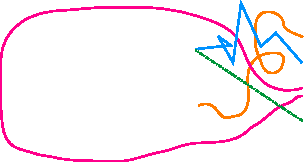
\includegraphics{images/wonky_lines.pdf}}
            ;
    \end{diagram}
\end{frame}

\newcommand{\col}[3]{(#2-row -| #3-col) node[#1] (#2-#3)}
\newcommand{\row}[4]{
    \col{tabular,replica}{#1}{new}{#2}
    \col{tabular,replica}{#1}{old}{#3}
    \col{}{#1}{descr}{#4}
}
\newcommand{\mozart}{Mozart \& 1756 \\}
\newcommand{\liszt}{Liszt \& 1811 \\}
\newcommand{\mahler}{Mahler \& 1860 \\}
\newcommand{\stevens}{Stevens \& 1948 \\}
\newcommand{\islam}{Islam \& 1948 \\}
\newcommand{\mms}{\mozart\mahler\stevens}
\newcommand{\bls}{Bach \& Germany \\ Liszt \& Hungary \\ Stevens \& England \\}
\begin{frame}[noframenumbering]
    \frametitle{Strange, but true}
    \scriptsize
    \begin{diagram}
        \path
            coordinate (heading-row)
            ++(0,-3em) coordinate (insert-row)
            ++(0,-5em) coordinate (typo-row)
            ++(0,-5em) coordinate (replace-row)
            ++(0,-5em) coordinate (name-row)
            ++(0,-5em) coordinate (bachbach-row)
            (heading-row) coordinate (old-col)
            ++(11em,0) coordinate (new-col)
            ++(10em,0) coordinate (descr-col)

            ($(old-col)!.5!(new-col)$) node {Alignment}
            \col{}{heading}{descr}{What Changed}
            \row{insert}  {\mms}                {\mozart\stevens}                   {insert Mahler}
            \row{typo}    {\mms}                {\mozart Maller \& 1860 \\ \stevens}{correct typo}
            \row{replace} {\mms}                {\mozart\liszt\stevens}             {replace a composer}
            \row{name}    {\mozart\mahler\islam}{\mms}                              {name change}
            \row{bachbach}{\bls}                {\bls}                              {replace Bach with son}
            ;
        \foreach \name/\conns in {
            insert/{1/1,3/2},
            typo/{1/1,2/2,3/3},
            replace/{1/1,3/3},
            name/{1/1,2/2,3/3},
            bachbach/{2/2,3/3}%
            }
            \foreach \i/\j in \conns
                \draw[thick] (\name-new-\i-1.west) -- (\name-old-\j-2.east);
    \end{diagram}
\end{frame}

\begin{frame}[noframenumbering]
    \frametitle{Future work}
    \begin{itemize}
        \item Hyperlenses: multi-repository lenses
        \item Transforming string edits into structured edits
        \item Further exploration of the possible edit lenses
        \item More breadth in the algebraic study of edit lenses
        \item Many ideas for applications
        \item Others: variations of the behavioral laws, typed edits,
            asymmetric edit lenses, connections between various lens
            frameworks, automatic weight function discovery
    \end{itemize}
\end{frame}

% TODO: perhaps make this a table with a tad more info?
\begin{frame}[noframenumbering]
    \frametitle{Potential application areas}
    \begin{itemize}
        \item Filesystem synchronization
        \item Text editing (decoding, parsing, highlighting)
        \item GUI internals
        \item Extensions of Boomerang, Augeas, Forest
        \item Many-directional spreadsheet
        \item Relational database
        \item Bidirectional Datalog
        \item Server/client applications (e.g. on mobile phones)
        \item Software model transformations
    \end{itemize}
\end{frame}

\end{document}
outline proposal
-  5: background + motivation
    - keep two pieces of data in synch, even though they are stored in a
      different format or have slightly different ``stuff'' inside
    - design transformation pairs in tandem
    - perhaps a bit of history? databases+complements; lenses and subsequent
      bloom of research; dissatisfaction with laws/asymmetry/alignment
-  5: scope of my work + the thesis + my contributions
    - contributions:
        - framework that supports symmetry, alignment, performance
        - algebraic study of the framework + an inhabiting syntax
        - prototype implementation
- 25: deep drill into something technical and cool; possibilities:
    - containers + container mapping + how alignment is solved with the edit
      language for containers; perhaps leading to container reshaping lens;
      perhaps coming from discussion of why recursive types are hard to
      design edit languages for
        - skip the lenses, talk just about edit languages to begin with
        - (free) edit monoid for products
        - (free) edit monoid for sums
        - make a couple attempts at an edit monoid for recursive types
        - notice that what we really want is some concept of a pointer into
          these structures
        - so model it that way explicitly, use containers
        - (free) edit monoid for containers
        - mapping lens for containers
        - observe how alignment is handled
        - discuss reshaping lens
    - the category of (edit) lenses, the machinery needed to make it be a
      category, what structure you get and don't (and why), what open
      questions this settles/insight this gives
    - behavioral laws: why the old ones don't cut it and how our
      monoid-based ones help; observation that partition is tricky and may
      require lax laws and what this tells us about the partition lens
    - possibly: the monoid isomorphism route to lenses (i.e. start with
      isomorphisms, see why they are too strong, see how to relax them, then
      add complements; can also discuss the ``one module per type''
      philosophy along the way to motivate adding complements vs. choosing a
      different edit language when designing partition lens)
-  5: overview of all results
-  5: pop back up a level and give some perspective + summary
    - symmetric lenses: first framework to offer symmetry + serious study of
      composition and the associated machinery
    - edit lenses: add incremental operation, talk about the processing of
      alignment information
    - implementation: still need some theory about generating alignment
      information

BCP suggests: expect to spend 3-5ish on related work, and similar or a bit
less on future work

BCP says:
    * give some motivation/perspective... but make it quick; almost
      everybody in the audience has seen my talks before, so they know
      what's going on
    * plan to make it to the list of contributions within about five minutes
    * two purposes for the presentation; should heavily weight my efforts
      towards really satisfying the second goal
        * as a public announcement of the work I've done and contributions
          I've made
        * gives the committee a chance to solidify their understanding and
          opinions of my work
SCW says:
    * BUT the focus should be on what I have contributed; the
      history/perspective should be there so that it's clear what I've
      contributed to the historical understanding, the technical stuff
      should be there so they understand what I've contributed, etc.; the
      technical content isn't the focus, but a means to conveying the focus
    * also, re-expressed the preference for explaining one thing well, i.e.
      it's reasonable to skimp on old work in favor of a good, in-depth
      explanation of the newest work
    * she mentioned in passing something like, "maybe half the talk is on
      your newest technical work, and five minutes is on how that connects
      with older work"
SAZ says:
    * definitely reiterate the motivation for the work
    * explain contributions to someone already familiar with the work
    * very important: situate this work compared to other work
    * might want to give the committee an overview of what they asked for at
      the proposal and how I addressed those recommendations
SAZ suggested a rough timing outline:
    *  5min background + motivation
    *  5min scope of my work + the thesis + my contributions
    * 30min deep drill into something technical and cool
    *  5min pop back up a level and give some perspective + summary

Timings for practice run 140605
Vis 09   9:10:00 (Other models of edits)
Vis 10   9:14:45 (Modules)
Vis 11   9:17:00 (Monoids)
Vis 12   9:18:20 (Partiality)
         9:19:10
         9:22:40
Vis 13   9:23:30 (Data structures)
         9:24:30
         9:24:45
Vis 14   9:25:30 (Free monoids)
Vis 15   9:26:15 (Products)
Vis 16   9:27:15 (Sums)
Vis 17   9:31:00 (Sums, recap)
Vis 18   9:31:43 (Recursive types)
Vis 19   9:36:00 (Recursive types, take two)
Vis 20   9:37:30 (Containers instead of recursive types)
Vis 21   9:38:15 (Containers)
Vis 22   9:39:45 (Container restrictions)
Vis 23   9:42:30 (Container module)
Vis 34   9:45:00 (Container mapping lens)
Vis 25   9:46:20 (Alignment)
Vis 26   9:47:00 (Reshaping)
End      9:47:30

Timings for practice run 140611 (which included skipping many slides)
01-05:  7:48
06-10: 17:57
11-15: 10:33
16-20:  6:43
21-25:  6:55
26-28:  4:37
total: 54:33

Timings for practice run 140612 (only skipped slide 18):
01-05:  6:46
06-06:  4:48
07-11: 10:51
12-16:  8:46
17-21:  7:50
22-26:  6:44
total: 45:50
